% Source: graduate-coursework/Research/Intro_to_Agents/handouts/Part6_MultiTier_Architecture.tex

\documentclass[border=4pt]{standalone}
\usepackage{amsmath,amssymb,amsfonts}
\usepackage[T1]{fontenc}
\usepackage{graphicx}
\usepackage{lmodern}
\usepackage{tikz}
\usepackage{xcolor}
\usetikzlibrary{shapes,arrows.meta,positioning,calc,fit,backgrounds,chains,decorations.pathreplacing}

\definecolor{UofSCGarnet}{HTML}{73000a}
\definecolor{UofSCBlack}{HTML}{000000}
\definecolor{UofSCWhite}{HTML}{ffffff}
\definecolor{UofSCRose}{HTML}{CC2E40}
\definecolor{UofSCAtlantic}{HTML}{466A9F}
\definecolor{UofSCCongaree}{HTML}{1F414D}
\definecolor{UofSCHorseshoe}{HTML}{65780B}
\definecolor{UofSCGrass}{HTML}{CED318}
\definecolor{UofSCHoneycomb}{HTML}{A49137}
\definecolor{UofSC90Black}{HTML}{363636}
\definecolor{UofSC70Black}{HTML}{5C5C5C}
\definecolor{UofSC50Black}{HTML}{A2A2A2}
\definecolor{UofSCWarmGrey}{HTML}{676156}
\definecolor{UofSCSandstorm}{HTML}{FFF2E3}
\definecolor{UofSCDarkGarnet}{HTML}{570008}
\definecolor{UofSCAzalea}{HTML}{844247}

\tikzset{
    % Base node style
    basenode/.style={
        draw=UofSCBlack,
        fill=UofSCWhite,
        line width=0.8pt,
        minimum height=0.8cm,
        minimum width=2cm,
        align=center,
        font=\small
    },
    % Strategy layer style
    strategynode/.style={
        basenode,
        fill=UofSCGarnet,
        text=UofSCWhite,
        minimum height=1cm,
        minimum width=4cm
    },
    % Planning layer style
    planningnode/.style={
        basenode,
        fill=UofSCAtlantic,
        text=UofSCWhite,
        minimum height=0.9cm,
        minimum width=3.5cm
    },
    % Execution layer style
    execnode/.style={
        basenode,
        fill=UofSCCongaree,
        text=UofSCWhite,
        minimum height=0.8cm,
        minimum width=2.5cm
    },
    % Generic box
    genericbox/.style={
        basenode,
        minimum width=2.8cm
    },
    % Arrow styles (straight lines only)
    myarrow/.style={
        ->,
        >=Stealth,
        line width=0.8pt,
        draw=UofSCBlack
    },
    % Bidirectional arrow
    biarrow/.style={
        <->,
        >=Stealth,
        line width=0.8pt,
        draw=UofSCBlack
    },
    % Phase box style
    phasebox/.style={
        basenode,
        minimum width=3.5cm,
        minimum height=1.2cm,
        font=\small\bfseries
    },
    % Small box
    smallbox/.style={
        basenode,
        minimum width=1.5cm,
        minimum height=0.6cm,
        font=\scriptsize
    },
    % Leader node
    leadernode/.style={
        basenode,
        fill=UofSCGarnet,
        text=UofSCWhite,
        minimum width=3cm,
        minimum height=1cm
    },
    % Worker node
    workernode/.style={
        basenode,
        fill=UofSC70Black,
        text=UofSCWhite,
        minimum width=1.2cm,
        minimum height=0.7cm,
        font=\scriptsize
    }
}

\begin{document}
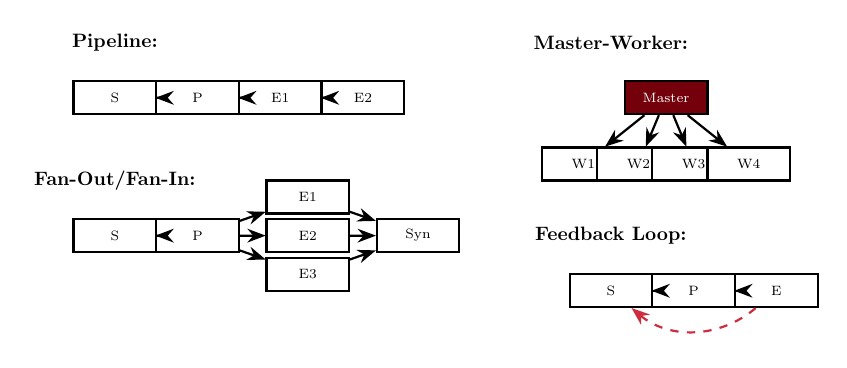
\begin{tikzpicture}[scale=0.7, transform shape]
        % Pattern 1: Pipeline
        \node[font=\bfseries] at (-4,5) {Pipeline:};
        \node[smallbox] (pa1) at (-4,4) {S};
        \node[smallbox] (pa2) at (-2.5,4) {P};
        \node[smallbox] (pa3) at (-1,4) {E1};
        \node[smallbox] (pa4) at (0.5,4) {E2};
        \draw[myarrow] (pa1) -- (pa2);
        \draw[myarrow] (pa2) -- (pa3);
        \draw[myarrow] (pa3) -- (pa4);

        % Pattern 2: Fan-Out/Fan-In
        \node[font=\bfseries] at (-4,2.5) {Fan-Out/Fan-In:};
        \node[smallbox] (fb1) at (-4,1.5) {S};
        \node[smallbox] (fb2) at (-2.5,1.5) {P};
        \node[smallbox] (fb3) at (-0.5,2.2) {E1};
        \node[smallbox] (fb4) at (-0.5,1.5) {E2};
        \node[smallbox] (fb5) at (-0.5,0.8) {E3};
        \node[smallbox] (fb6) at (1.5,1.5) {Syn};
        \draw[myarrow] (fb1) -- (fb2);
        \draw[myarrow] (fb2) -- (fb3);
        \draw[myarrow] (fb2) -- (fb4);
        \draw[myarrow] (fb2) -- (fb5);
        \draw[myarrow] (fb3) -- (fb6);
        \draw[myarrow] (fb4) -- (fb6);
        \draw[myarrow] (fb5) -- (fb6);

        % Pattern 3: Master-Worker
        \node[font=\bfseries] at (5,5) {Master-Worker:};
        \node[smallbox, fill=UofSCGarnet, text=white] (mw1) at (6,4) {Master};
        \node[smallbox] (mw2) at (4.5,2.8) {W1};
        \node[smallbox] (mw3) at (5.5,2.8) {W2};
        \node[smallbox] (mw4) at (6.5,2.8) {W3};
        \node[smallbox] (mw5) at (7.5,2.8) {W4};
        \draw[myarrow] (mw1) -- (mw2);
        \draw[myarrow] (mw1) -- (mw3);
        \draw[myarrow] (mw1) -- (mw4);
        \draw[myarrow] (mw1) -- (mw5);

        % Pattern 4: Feedback Loop
        \node[font=\bfseries] at (5,1.5) {Feedback Loop:};
        \node[smallbox] (fl1) at (5,0.5) {S};
        \node[smallbox] (fl2) at (6.5,0.5) {P};
        \node[smallbox] (fl3) at (8,0.5) {E};
        \draw[myarrow] (fl1) -- (fl2);
        \draw[myarrow] (fl2) -- (fl3);
        \draw[myarrow, dashed, color=UofSCRose] (fl3) to[bend left=40] (fl1);
    \end{tikzpicture}
\end{document}
